\documentclass[a4paper,12pt]{article}
%%% Работа с русским языком
\usepackage[unicode, pdftex]{hyperref}
\usepackage{cmap}					% поиск в PDF
\usepackage{mathtext} 				% русские буквы в формулах
\usepackage[T2A]{fontenc}			% кодировка
\usepackage[utf8]{inputenc}			% кодировка исходного текста
\usepackage[english,russian]{babel}	% локализация и переносы
\usepackage{indentfirst}
\frenchspacing


\renewcommand{\epsilon}{\ensuremath{\varepsilon}}
\renewcommand{\phi}{\ensuremath{\varphi}}
\renewcommand{\kappa}{\ensuremath{\varkappa}}
\renewcommand{\le}{\ensuremath{\leqslant}}
\renewcommand{\leq}{\ensuremath{\leqslant}}
\renewcommand{\ge}{\ensuremath{\geqslant}}
\renewcommand{\geq}{\ensuremath{\geqslant}}
\renewcommand{\emptyset}{\varnothing}

%%% Дополнительная работа с математикой
\usepackage{amsmath,amsfonts,amssymb,amsthm,mathtools} % AMS
\usepackage{icomma} % "Умная" запятая: $0,2$ --- число, $0, 2$ --- перечисление

%% Номера формул
%\mathtoolsset{showonlyrefs=true} % Показывать номера только у тех формул, на которые есть \eqref{} в тексте.
%\usepackage{leqno} % Нумереация формул слева

%% Свои команды
\DeclareMathOperator{\sgn}{\mathop{sgn}}

%% Перенос знаков в формулах (по Львовскому)
\newcommand*{\hm}[1]{#1\nobreak\discretionary{}
	{\hbox{$\mathsurround=0pt #1$}}{}}

%%% Работа с картинками
\usepackage{graphicx}  % Для вставки рисунков
%\graphicspath{{images/}{images2/}}  % папки с картинками
\setlength\fboxsep{3pt} % Отступ рамки \fbox{} от рисунка
\setlength\fboxrule{1pt} % Толщина линий рамки \fbox{}
\usepackage{wrapfig} % Обтекание рисунков текстом

%%% Работа с таблицами
\usepackage{array,tabularx,tabulary,booktabs} % Дополнительная работа с таблицами
\usepackage{longtable}  % Длинные таблицы
\usepackage{multirow} % Слияние строк в таблице

%%% Теоремы
\theoremstyle{plain} % Это стиль по умолчанию, его можно не переопределять.
\newtheorem{theorem}{Теорема}[section]
\newtheorem{proposition}[theorem]{Утверждение}

\theoremstyle{definition} % "Определение"
\newtheorem{corollary}{Следствие}[theorem]
\newtheorem{problem}{Задача}[section]

\theoremstyle{remark} % "Примечание"
\newtheorem*{nonum}{Решение}

%%% Программирование
\usepackage{etoolbox} % логические операторы

%%% Страница
\usepackage{extsizes} % Возможность сделать 14-й шрифт
\usepackage{geometry} % Простой способ задавать поля
\geometry{top=25mm}
\geometry{bottom=35mm}
\geometry{left=25mm}
\geometry{right=20mm}
%
\usepackage{fancyhdr} % Колонтитулы
\pagestyle{fancy}
%\renewcommand{\headrulewidth}{0pt}  % Толщина линейки, отчеркивающей верхний колонтитул
% 	\lfoot{Нижний левый}
% 	\rfoot{Нижний правый}
% 	\chead{Верхний в центре}
% 	\lhead{Верхний левый}
%	\cfoot{Нижний в центре} % По умолчанию здесь номер страницы
\usepackage{lastpage}
\fancyhead[R]{РЭМ. Группа Б04-004}
\fancyhead[L]{}
\fancyhead[C]{}

\usepackage{setspace} % Интерлиньяж (расстояние между строками)
%\onehalfspacing % Интерлиньяж 1.5
%\doublespacing % Интерлиньяж 2
%\singlespacing % Интерлиньяж 1

\usepackage{lastpage} % Узнать, сколько всего страниц в документе.




\usepackage[usenames,dvipsnames,svgnames,table,rgb]{xcolor}
\hypersetup{				% Гиперссылки
	unicode=true,           % русские буквы в раздела PDF
	pdftitle={Заголовок},   % Заголовок
	pdfauthor={Автор},      % Автор
	pdfsubject={Тема},      % Тема
	pdfcreator={Создатель}, % Создатель
	pdfproducer={Производитель}, % Производитель
	pdfkeywords={keyword1} {key2} {key3}, % Ключевые слова
	colorlinks=true,       	% false: ссылки в рамках; true: цветные ссылки
	linkcolor=red,          % внутренние ссылки
	citecolor=black,        % на библиографию
	filecolor=magenta,      % на файлы
	urlcolor=cyan           % на URL
}


%\usepackage[style=authoryear,maxcitenames=2,backend=biber,sorting=nty]{biblatex}

\usepackage{multicol} % Несколько колонок

\usepackage{tikz} % Работа с графикой
\usepackage{pgfplots}
\usepackage{pgfplotstable}
\usepackage{floatrow}
\DeclareFloatSeparators{mysep}{\hspace{3cm}}
\thisfloatsetup{floatrowsep=mysep}


\begin{document}
	\newpage
	\section{Введение}
	Растровая электронная микроскопия- современный метод изучения поверхности твёрдых тел. В растровой микроскопии, в отличии от просвечивающей, обычно не требуется никакой предварительной подготовки поверхности, а также возможен анализ объемных объектов. Ещё одно ее преимущество- большая глубина резкости, получающаяся за счет большого фокусного расстояния последней линзы.
	
	Растровая электронная микроскопия получает изображение за счет бомбардировки поверхности сфокусированным электронным лучом. Выбитые электронным лучом вторичные электроны регистрируются детектором электронов. На основе этого создается изображение интенсивности вторичной эмиссии. Так как коэффициент вторичной эмиссии зависит от угла падения первичных электронов, это изображение определяется рельефом исследуемой поверхности.
	\section{Устройство и работа растрового электронного микроскопа}
	Микроскоп, изучаемый в ходе данной работы, позволяет вести наблюдения образца в трех основных режимах: во вторичных электронах, в отраженных электронах, в рентгеновских лучах. Для первых двух режимов оптимальный ток с точки зрения точности результатов составляет 1-1000 пА, при рентгеновском микроанализе оптимальным считается ток зонда порядка 100 нА. Поэтому ток зонда микроскопа изменяется в широких пределах.
	
	Структурная схема микроскопа дана на рис.1. Электронная пушка, которая представляет собой катод на эффекте Шоттки, является источником электронов. Затем происходит ускорение и первичная фокусировка пучка с помощью цилиндра Венельта и кольцевого анода. Далее следует система электронной оптики, которая формирует узкий зонд, а также позволяет отклонять его в сторону, направляя в определенные точки образа. Во внутренних областях колонны поддерживается вакуум, чтобы избежать рассеяния электронов и порчи катода.
	\begin{figure}[H]
		\centering
		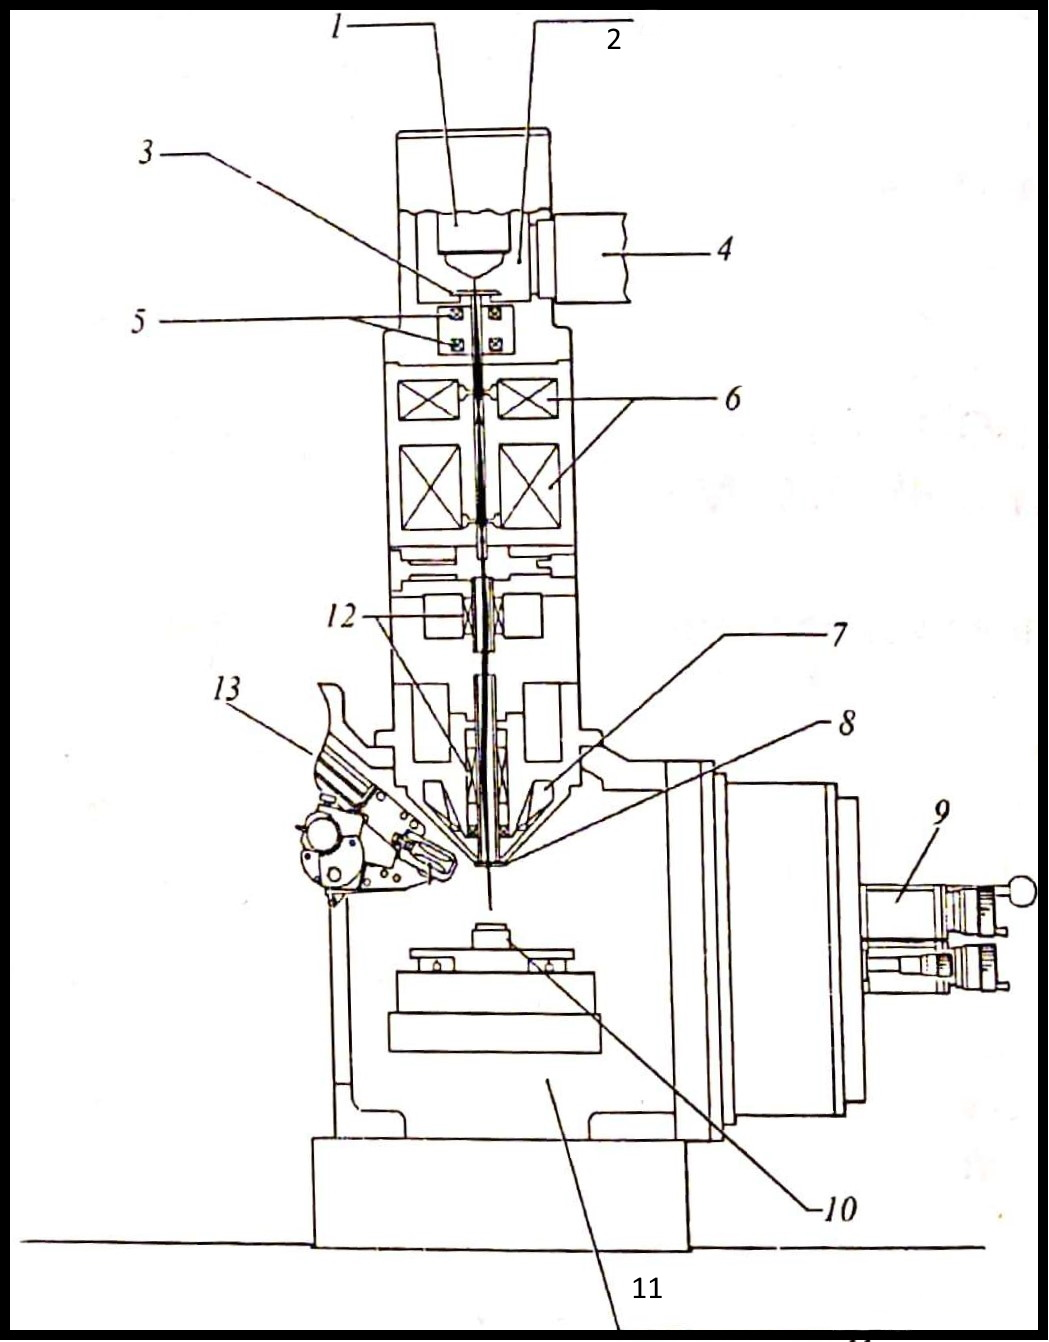
\includegraphics[scale=0.3]{pic1.jpg}
		\caption{Общая схема растрового электронного микроскопа. 1-электронная пушка; 2-камера электронной пушки; 3-анод; 4-вакуумная магистраль; 5-юстировочные катушки; 6-конденсаторные линзы; 7-объектная линза; 8-детектор упруго отраженных электронов; 9-система позиционирования образцов; 10-держатель образцов; 11-основная вакуумная камера; 12-сканирующие катушки; 13-рентгеновский спектрометр}
		\label{pic1}
	\end{figure}

\begin{figure}[H]
	\centering
	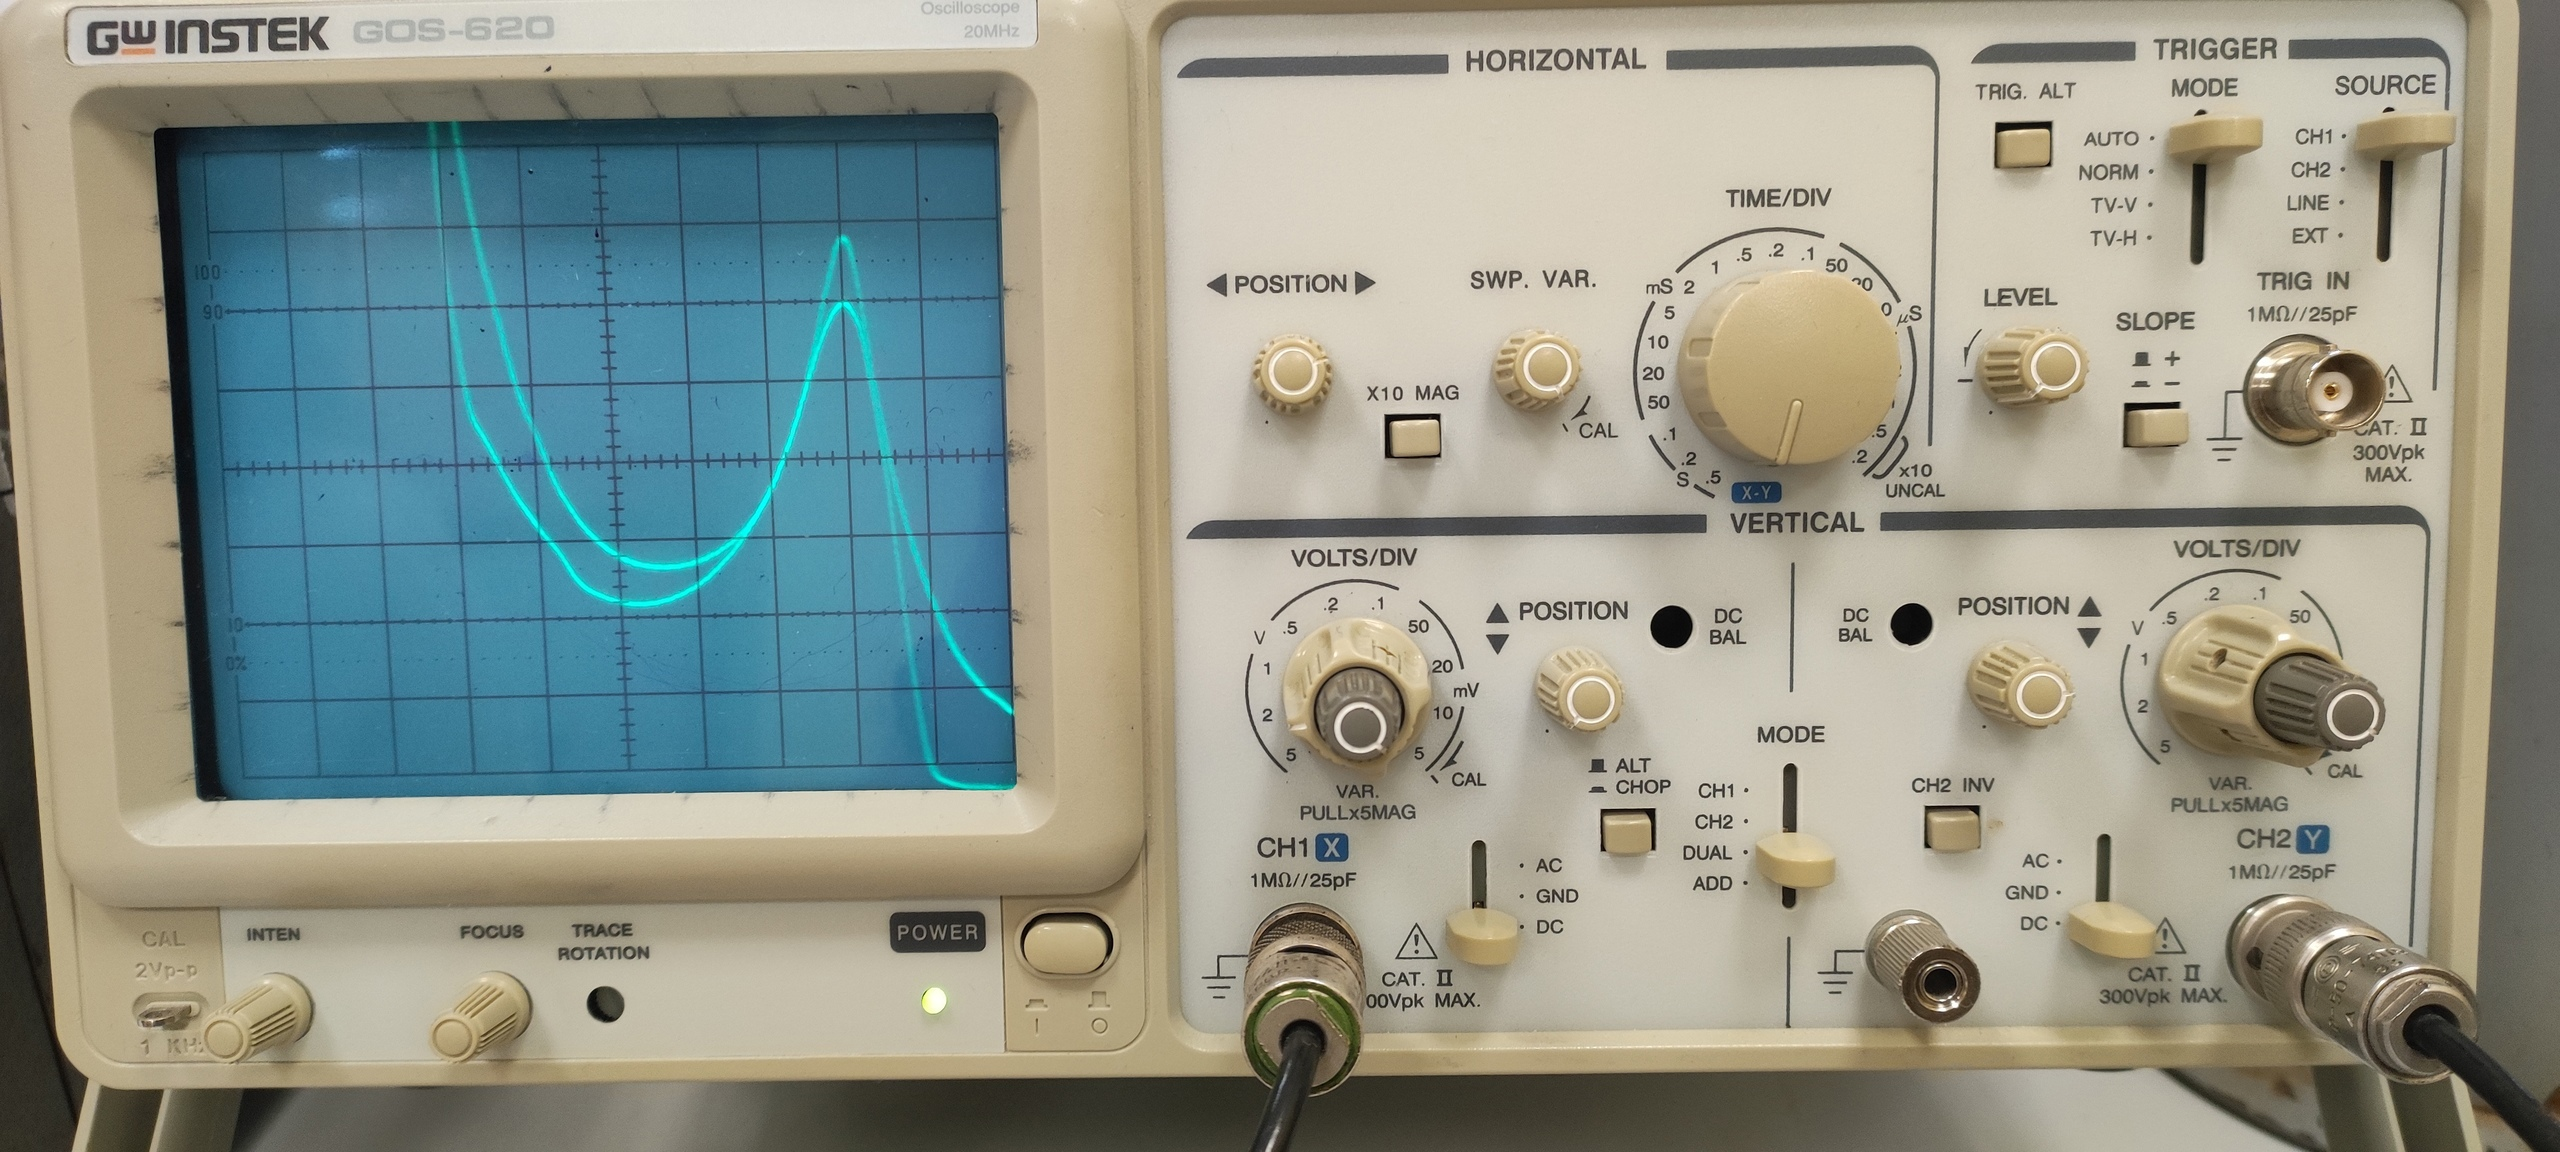
\includegraphics[scale=0.13]{pic2.jpg}
	\caption{Фотография экспериментальной установки}
	\label{pic2}
\end{figure}
Образец крепится на специальном держателе, в нашем случае с помощью проводящего углеродного скотча, позволяющем максимально удобно оперировать с образцами в процессе работы. Образец окружен детектирующей аппаратурой - детектором отраженных электронов, детектором истинно вторичных электронов, рентгеновским спектрометром. 
\section{Ход работы}
\subsection{Подготовка к измерениям}
Для проведения микроскопии требуется поместить образец в основную камеру без нарушения вакуума. Для этого предназначена система позиционирования образцов 9. Система напоминает шлюз космического корабля. Давление в шлюзе поднимается до атмосферного путем открытия электронного клапана, после чего в него помещается держатель с образцами. В нашей работе это часть крыла мотылька и бабочки, таблетка, состоящая из двух неизвестных металлов, два монокристаллических образца кремния, пенопластовый шарик. Шлюз закрывается, начинается откачка шлюзовой камеры с образцами. 


В установке используется один форвакуумный насос, поэтому, чтобы не испортить вакуум в основной вакуумной камере, она отделяется заслонкой от насоса и начинается откачка. Когда давления в шлюзе и основной камере сравняются - система откроет соединяющий клапан и давления выравняются. 

После достижения рабочего давления ($ \approx 1\e{-4}\s Па $) и открытия клапана, соединяющего шлюз с основной камерой, образцы перемещаются в рабочую зону с помощью рычага. 

В программном обеспечении устанавливается параметр offset=9 мм, отвечающий за высоту таблетки с образцами. Можно приступать к микроскопии. 
\subsection{Микроскопия}
\subsubsection{Крыло бабочки}
\begin{figure}[H]
	\centering
	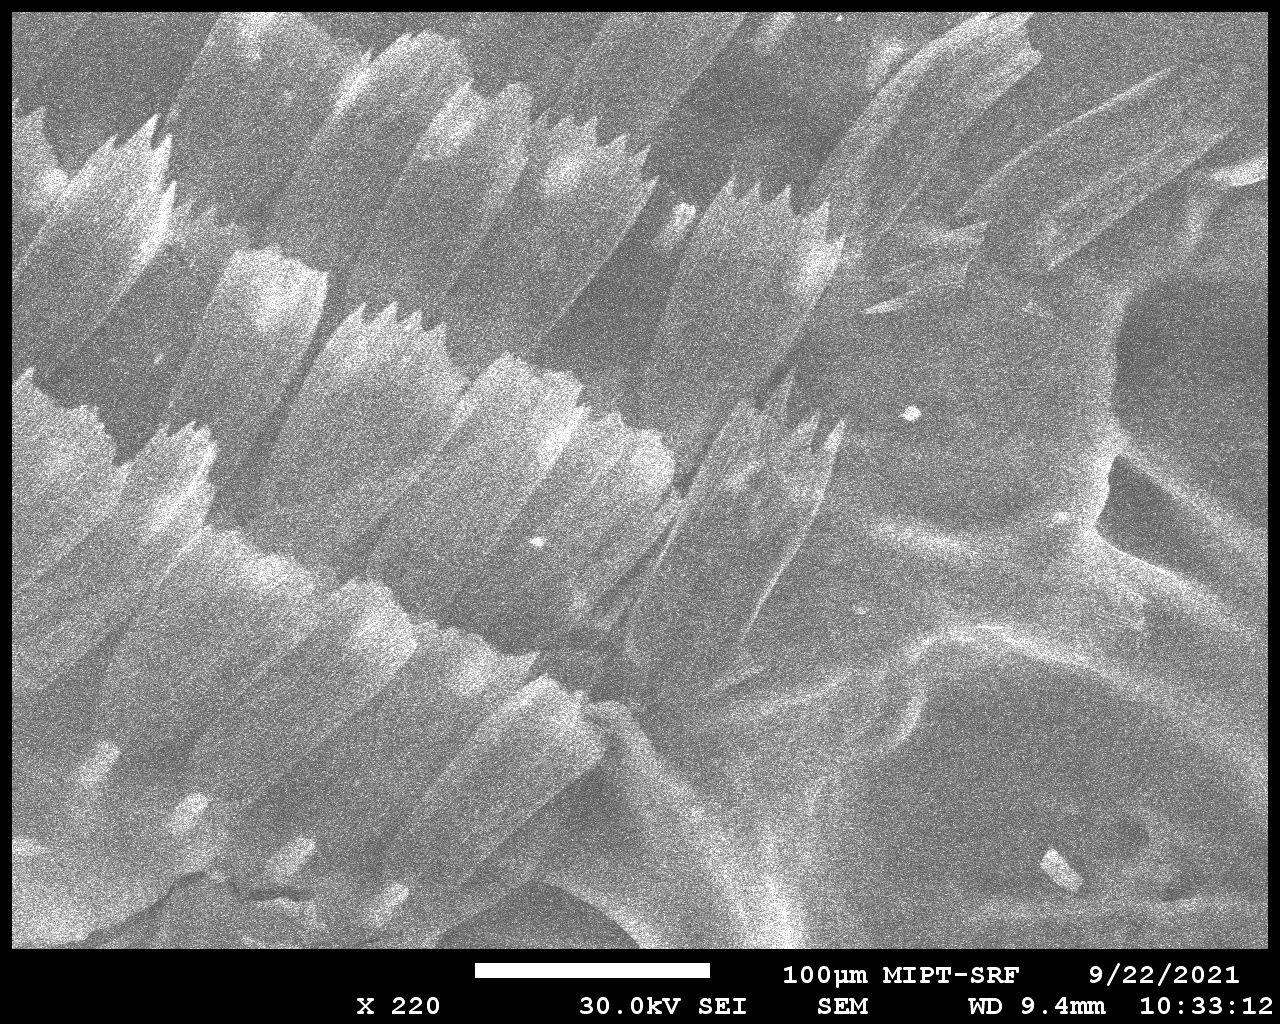
\includegraphics[scale=1.3]{pic3.jpg}
	\caption{Крыло бабочки. Быстрый режим сканирования}
	\label{pic3}
\end{figure}
На \picref{pic3} изображен результат сканирования крыла бабочки в режиме истинно вторичных электронов (SEI), полученное в реальном времени. Изображение зашумлено, однако отчетливо видны отдельные чешуйки ($ \approx 100\s мкм $) из которых состоит крыло.
\begin{figure}[H]
	\centering
	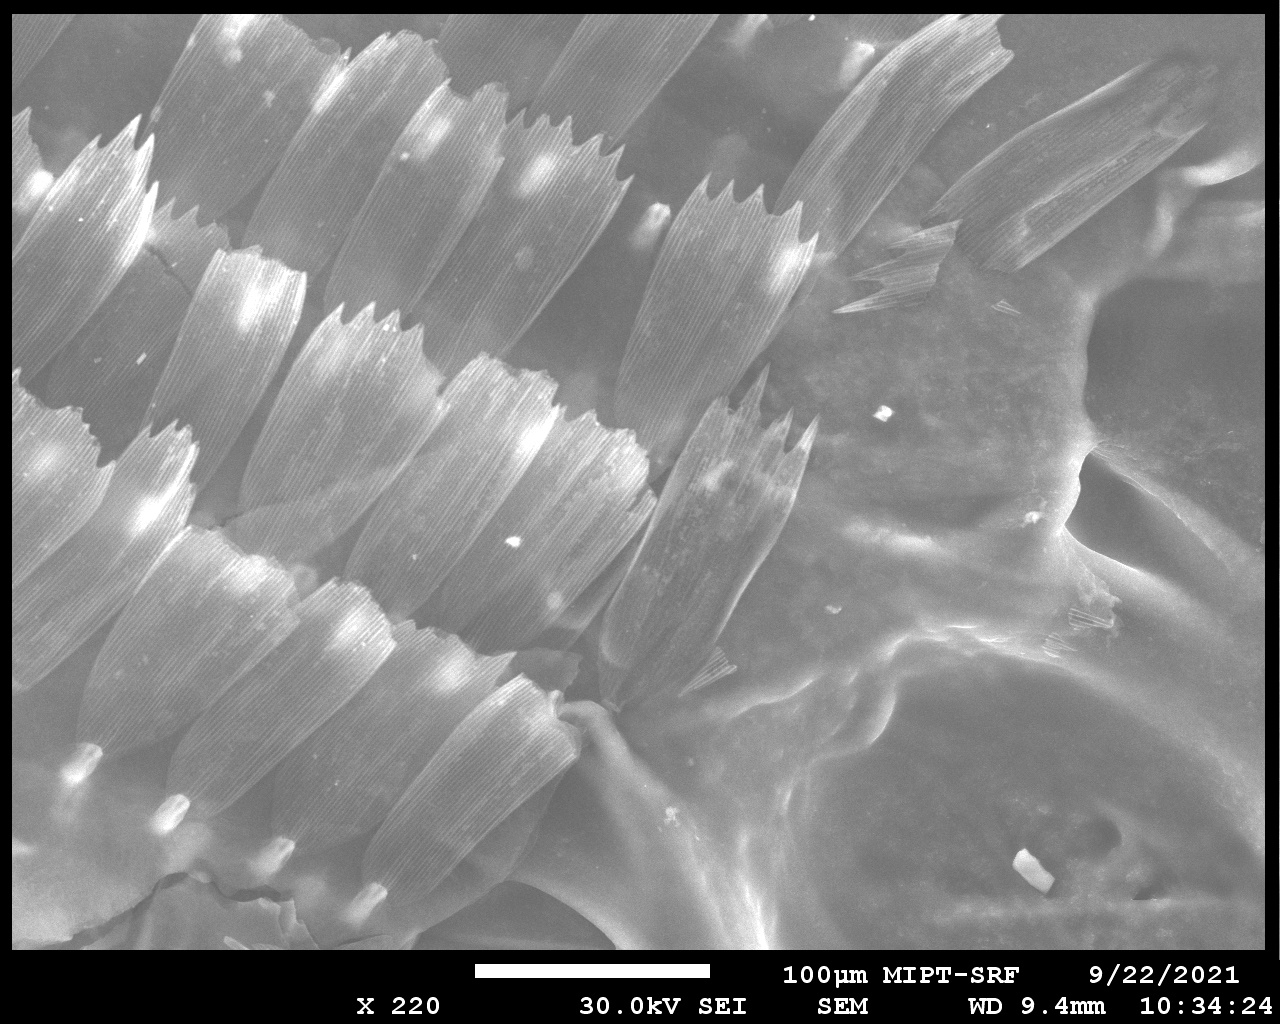
\includegraphics[scale=1.3]{pic4.jpg}
	\caption{Крыло бабочки. Медленный режим сканирования}
	\label{pic4}
\end{figure}
Для получения более детального изображения, следует понизить скорость сканирования \picref{pic4}. За счет этого уменьшается относительная интенсивность шумов, изображение проясняется и становится возможным наблюдать сложную структуру самой чешуйки, состоящей из множества канальцев.

При приближенном рассмотрении одного из таких канальцев \picref{pic5} становится видна пористая структура, заполняющая пространство между направляющими канальцами. Характерный размер пор составляет $ \approx 500\s нм $, что соизмеримо с длиной волны видимого излучения. За счет этого крыло бабочки приобретает свой переливающийся окрас, так как подобный размер структур создает условия для дифракции видимого света, что и приводит к окрашиванию крыла.
\begin{figure}[H]
	\centering
	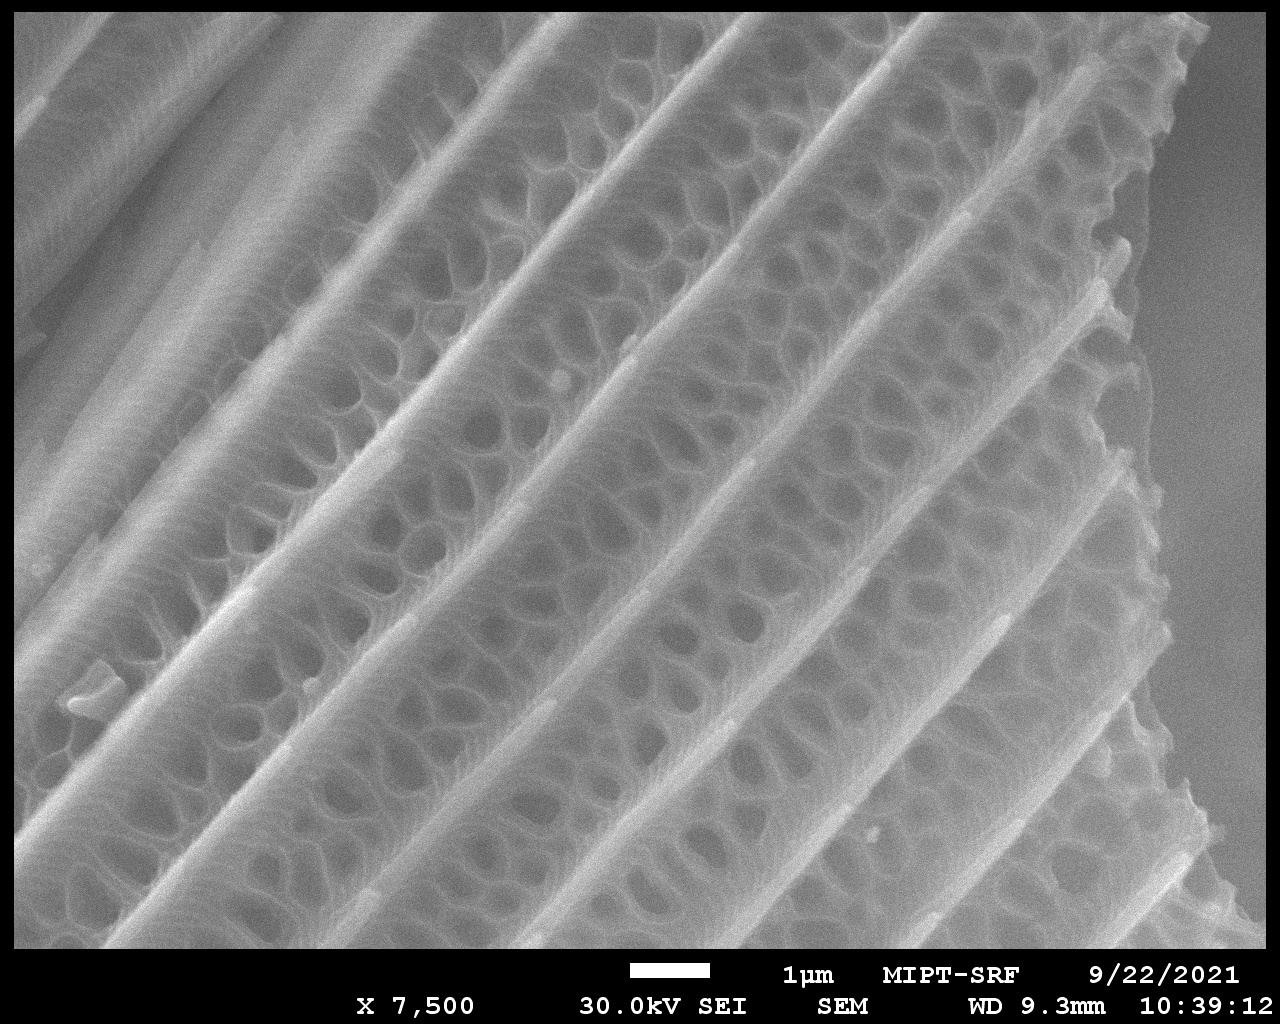
\includegraphics[scale=1.3]{pic5.jpg}
	\caption{Крыло бабочки. Структура отдельной чешуйки}
	\label{pic5}
\end{figure}
\subsubsection{Таблетка из двух металлов}

\begin{figure}[H]
	\centering
	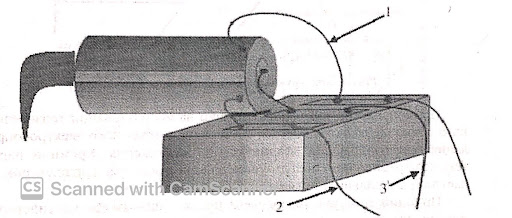
\includegraphics[scale=1.3]{pic6.jpg}
	\caption{Таблетка из двух металлов}
	\label{pic6}
\end{figure}
На \picref{pic6} изображен контрольный скан таблетки в режиме вторичных электронов. На скане присутствует информация как о рельефе, так и о элементном составе образца, но в перемешанной и трудноинтерпретируемой форме. Для получения раздельной информации о рельефе и о составе образца, переключимся в режим сбора упруго отраженных электронов (BSE). Для этого в основную камеру необходимо ввести датчик упруго отраженных электронов, имеющий форму двухсекционного диска. 

\begin{figure}[H]
	\centering
	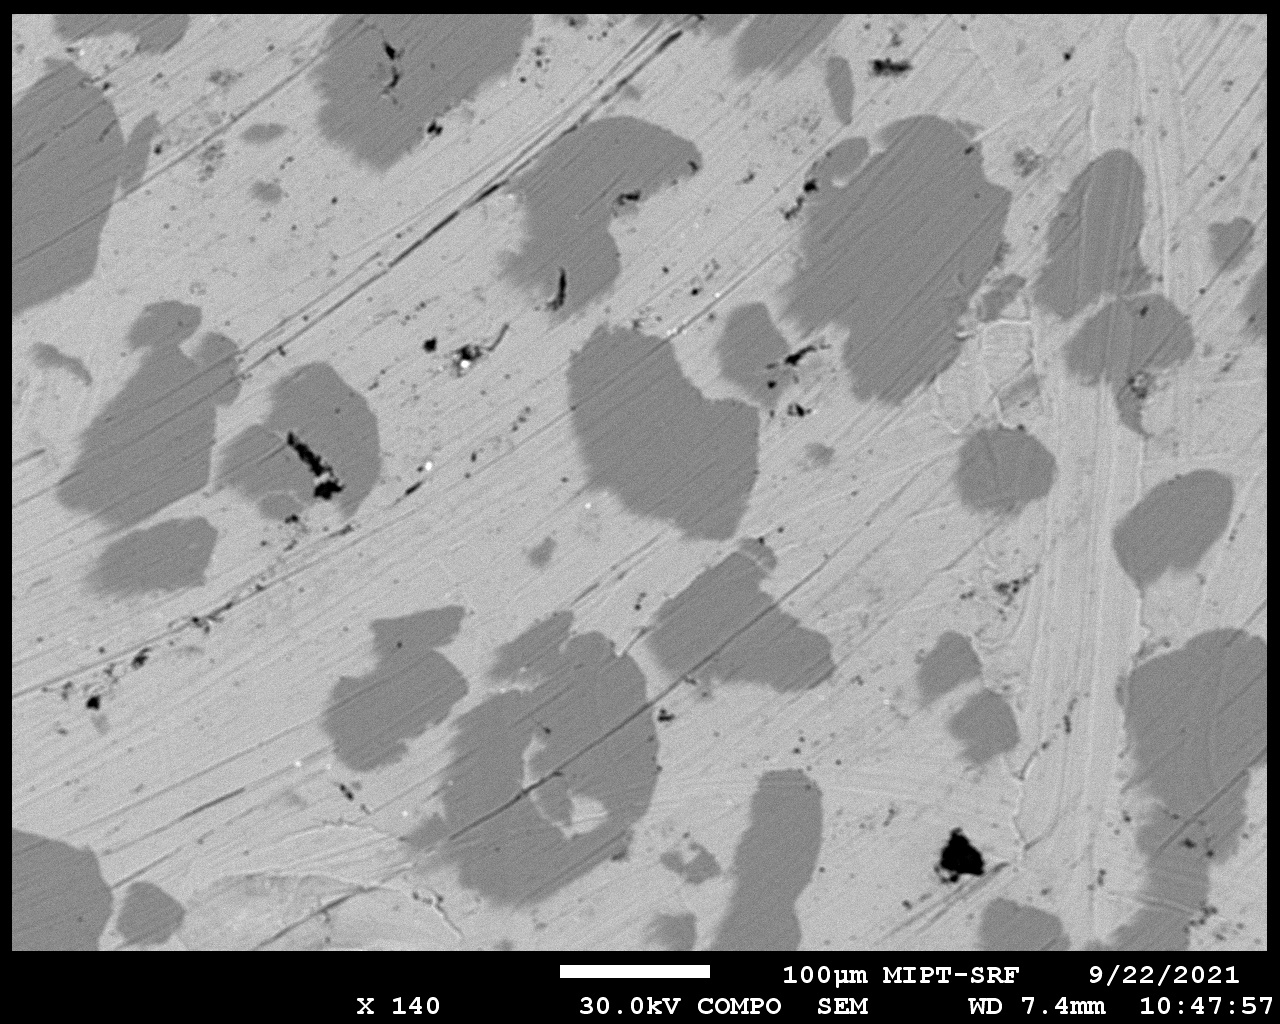
\includegraphics[scale=1]{pic7.jpg}
	\caption{Таблетка. Z-контраст}
	\label{pic7}
\end{figure}
\begin{figure}[H]
	\centering
	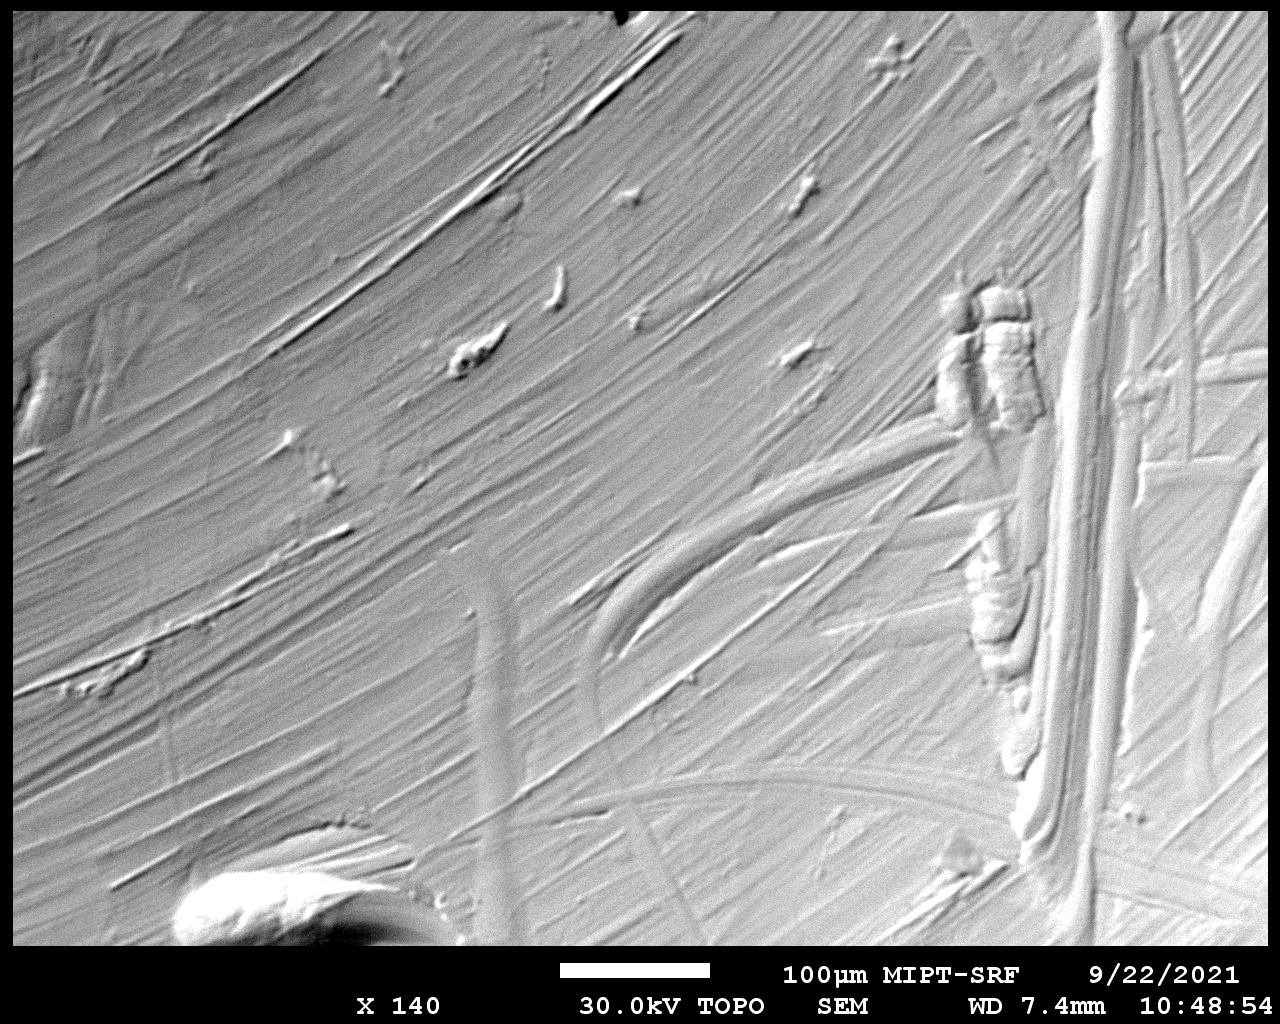
\includegraphics[scale=1]{pic8.jpg}
	\caption{Таблетка. Топологический контраст}
	\label{pic8}
\end{figure}

В режиме Z-контраста \picref{pic7}  отчетливо видны темные пятна- участки с другим химическим составом. Особенности рельефа также заметны, но в меньшей степени. В режиме топологического контраста \picref{pic8} отчетливо видны все особенности рельефа, а информация о различном составе полностью отсутствует.

Для определения элементного состава образца, воспользуемся рентгеноспектральным анализом. 

\begin{figure}[H]
	\centering
	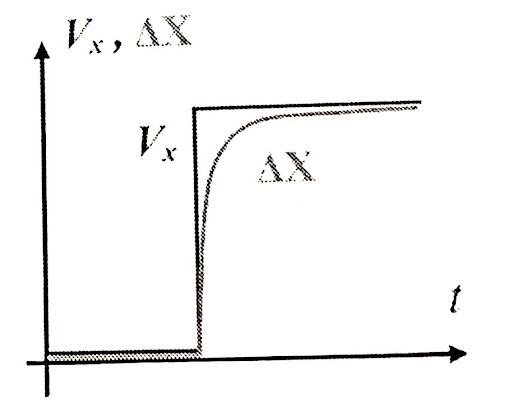
\includegraphics[scale=0.6]{pic9.jpg}
	\caption{Спектр рентгеновского излучения}
	\label{pic9}
\end{figure} 
\begin{figure}[H]
	\centering
	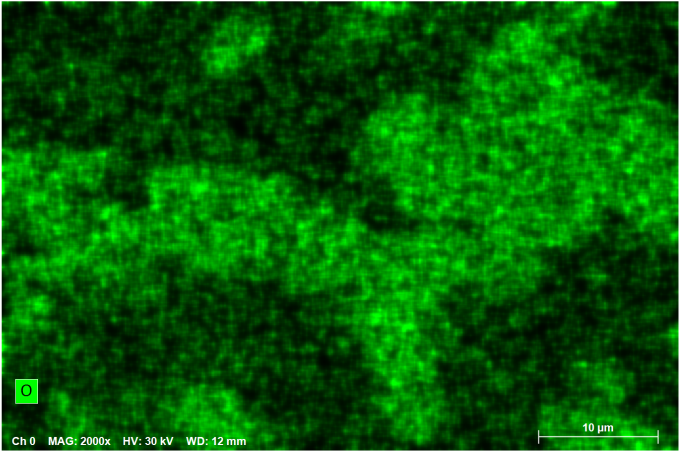
\includegraphics[scale=0.6]{pic10.png}
	\caption{Таблетка. Карта кислорода}
	\label{pic10}
\end{figure}
\begin{figure}[H]
	\centering
	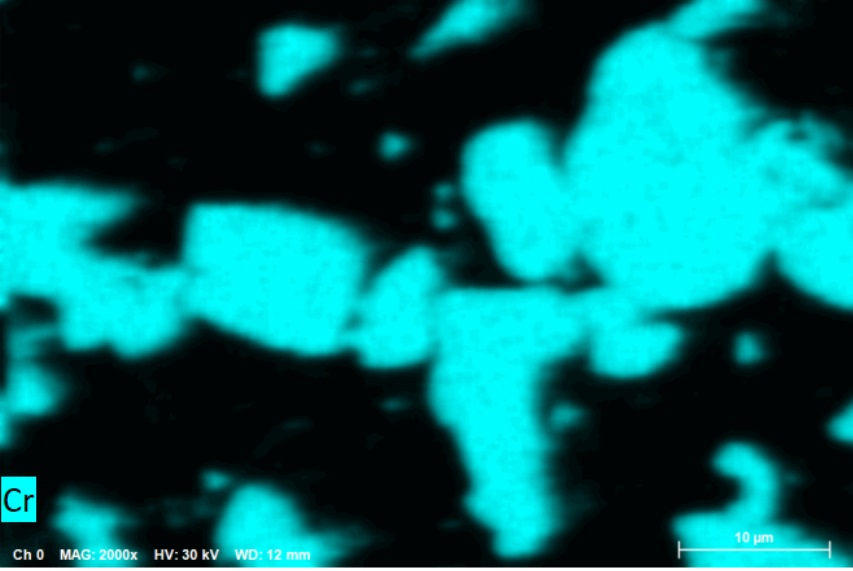
\includegraphics[scale=0.6]{pic11_2.jpg}
	\caption{Таблетка. Карта хрома}
	\label{pic11_2}
\end{figure}
\begin{figure}[H]
	\centering
	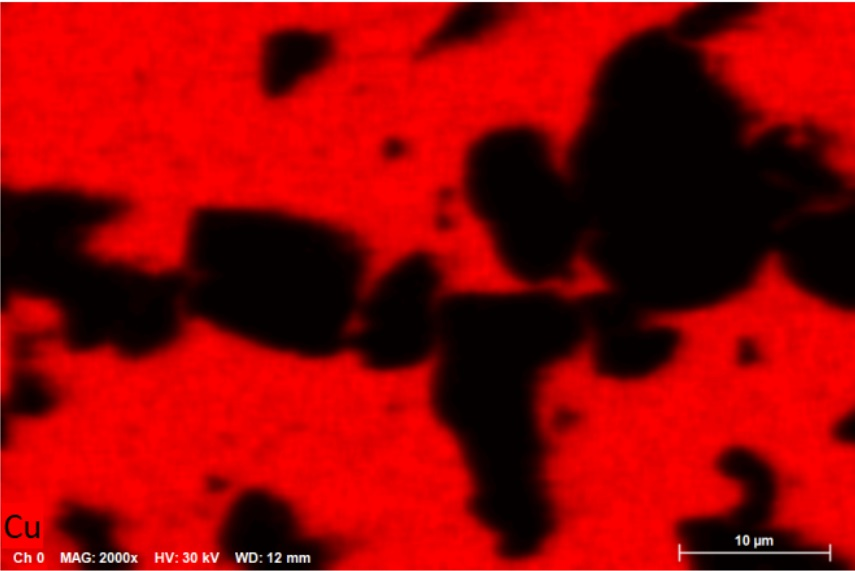
\includegraphics[scale=0.6]{pic11_1.jpg}
	\caption{Таблетка. Карта меди}
	\label{pic11_1}
\end{figure}

На спектрограмме отчетливо видны пики кислорода, углерода,хрома и меди. Кислород и углерод попали на образец из внешней среды. Хром и медь - материалы из которых изготовлена таблетка. Чтобы в этом убедиться, рассмотрим карту меди и хрома(рис.11 и рис.12). Образец состоит из меди с вкраплениями хрома. 

Заметим также один любопытный эффект. На карте кислорода(рис.10) области повышенной концентрации кислорода соответствуют вкраплениям хрома. Это можно объяснить повышенной адсорбционной способностью хрома по сравнению с кислородом или разной скоростью/толщиной образования оксидной пленки на поверхности металлов. 

\subsubsection{Монокристаллы кремния}
Для исследования образцов кремния, зафиксируем электронный луч в одной точке, заставив его освещать образец под разными углами. На рис.13 видны симметричные полосы, причем на первом образце их 4, а на втором 3. Эти полосы - направления вдоль граней монокристалла, появившиеся в результате эффекта каналирования первичных электронов.

На рисунке 13 наблюдается симметрия 6-го порядка. Это объясняется тем, что кристалл выращен таким образом, что его вершина направлена вверх 

На рисунке 14 более узкие полосы соответствуют основным направлениям граням куба, а более широкие- диагональные направления

\begin{figure}[H]
	\centering
	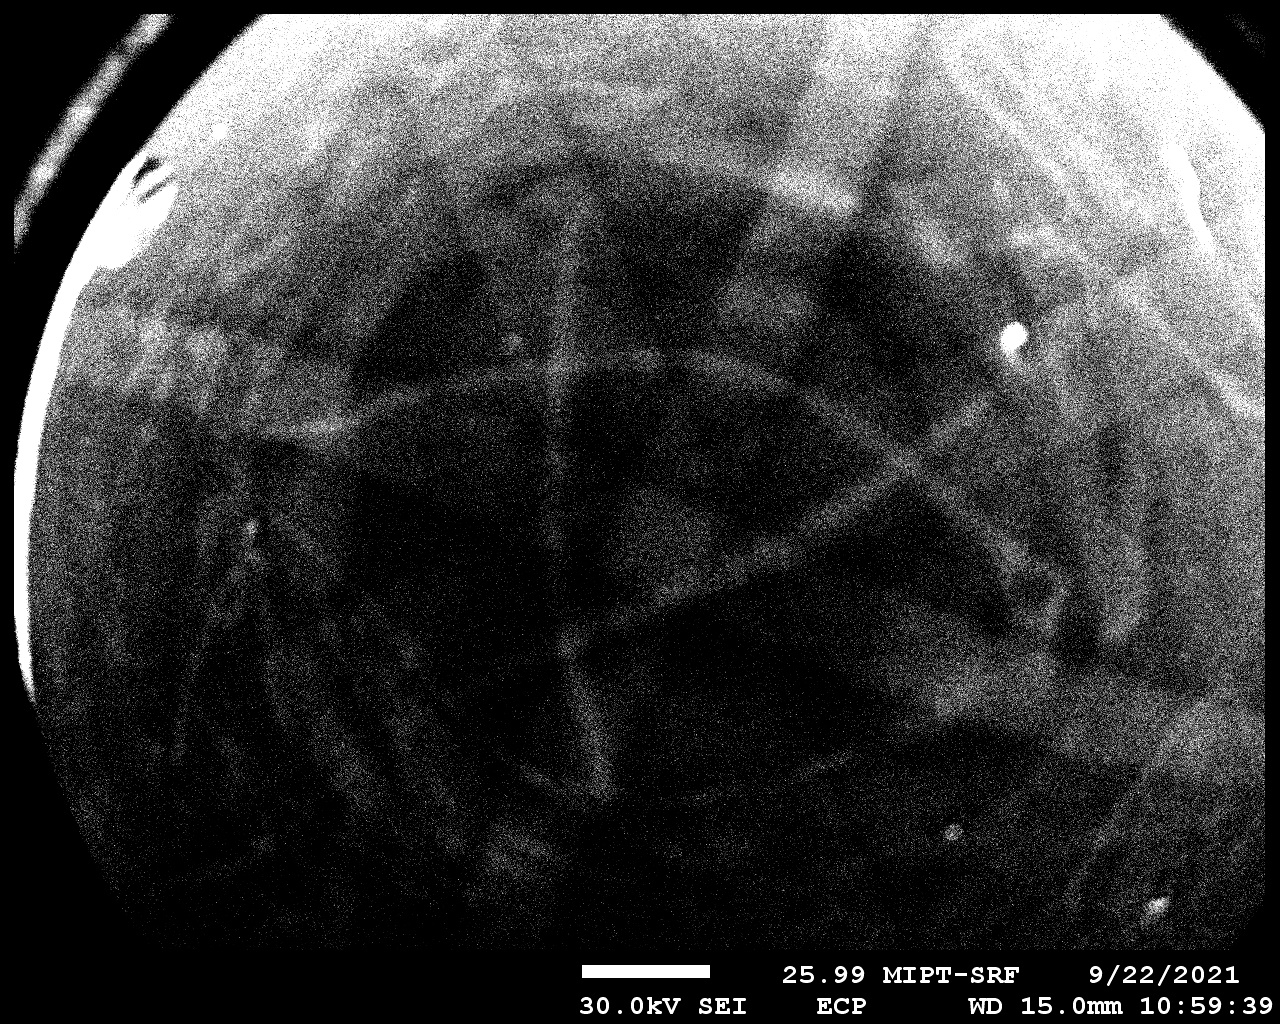
\includegraphics[scale=1]{pic12.jpg}
	\caption{Монокристалл кремния вершиной вверх}
	\label{pic12}
\end{figure}

\begin{figure}[H]
	\centering
	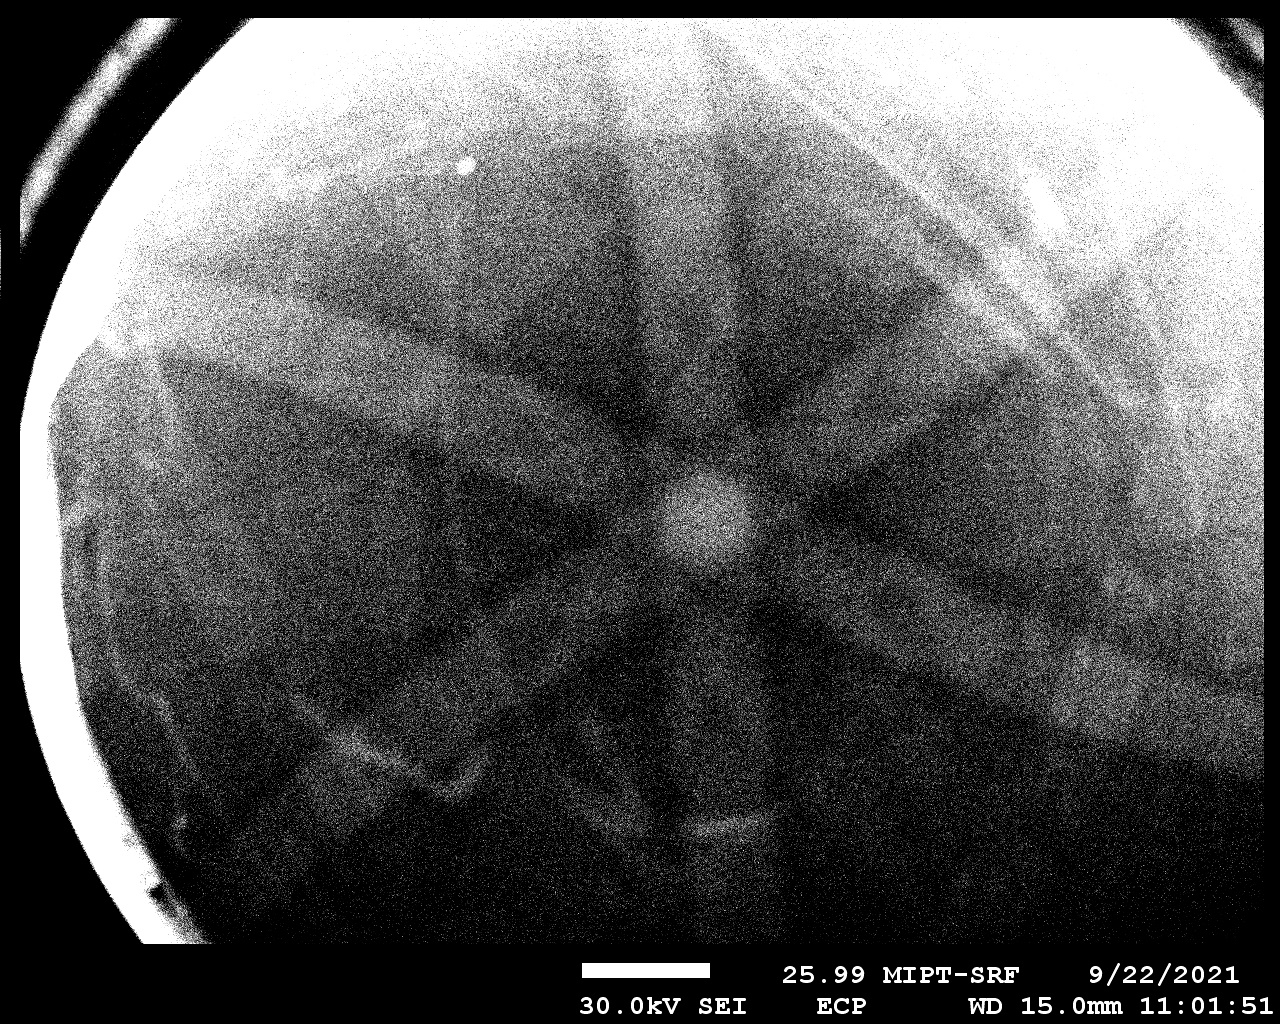
\includegraphics[scale=0.3]{pic13.jpg}
	\caption{Монокристалл кремния гранью вверх}
	\label{pic12}
\end{figure}

\subsubsection{Пенопласт}
Отличительным свойством этого образца \picref{pic14} является то, что это диэлектрик. Вследствие этого, в процессе сканирования, на образце накапливается отрицательный заряд, который своим полем начинает искажать траекторию движения первичных электронов, что ведет к деформации изображения, а именно к его сжатию.


\begin{figure}[H]
	\centering
	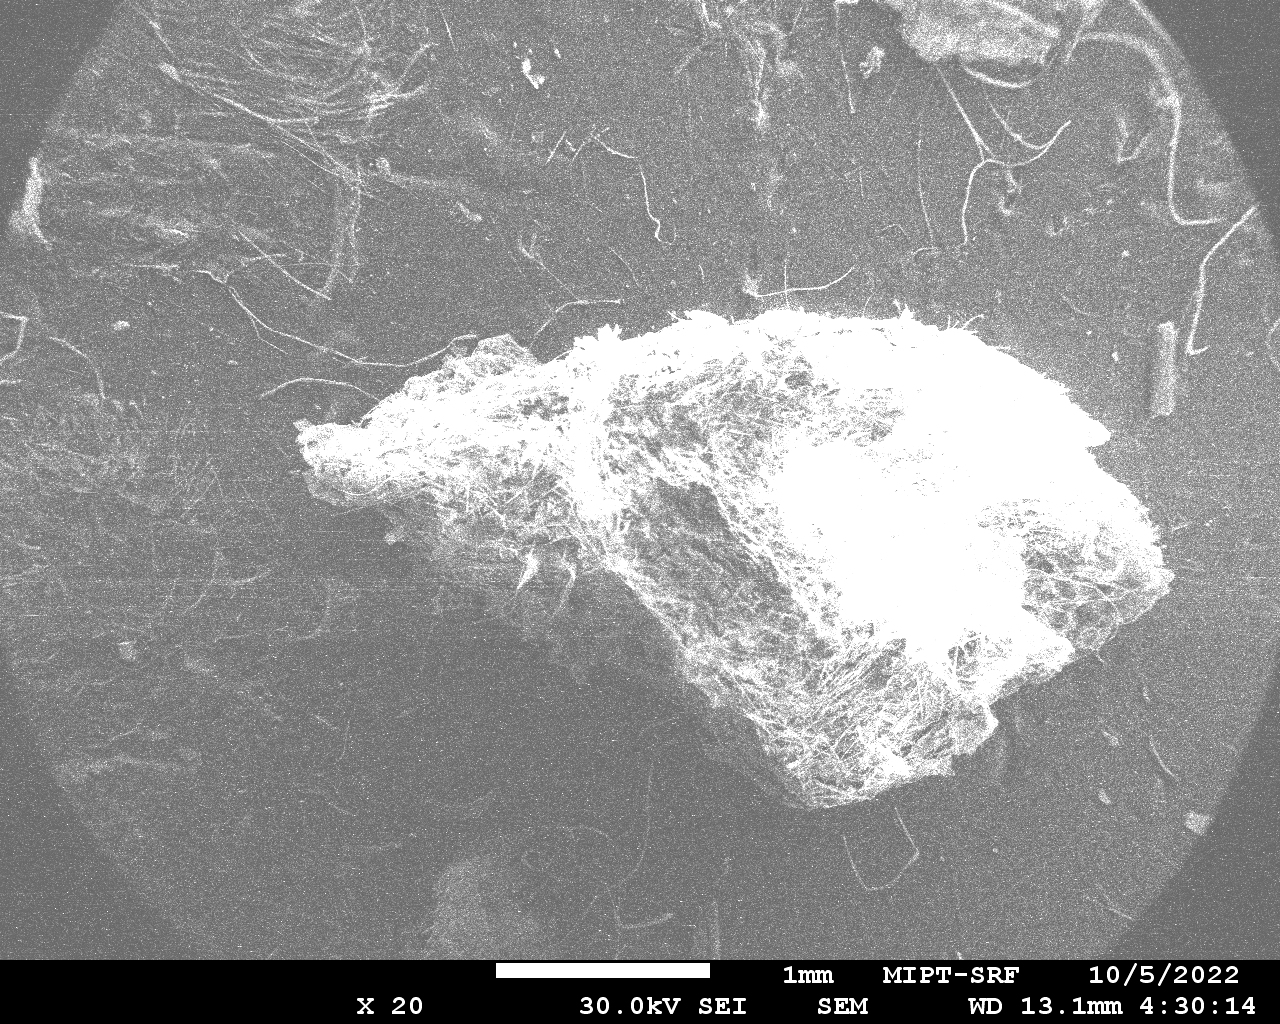
\includegraphics[scale=1]{pic14.jpg}
	\caption{Пенопласт}
	\label{pic14}
\end{figure}

Можно пронаблюдать интересный эффект, если начать постепенно понижать энергию первичных электронов. Изображение вначале деформируется до неузнаваемости, а затем в нем начнет проявляться изображение верхней внутренней части микроскопа- отверстие колонны, детектор вторичных электронов, детектор упруго отраженных электронов и рентгеновский детектор. Яркость детектора на изображении может объяснятся тем, что в этих точках изображения в него попадают первичные электроны напрямую.
\begin{figure}[H]
	\centering
	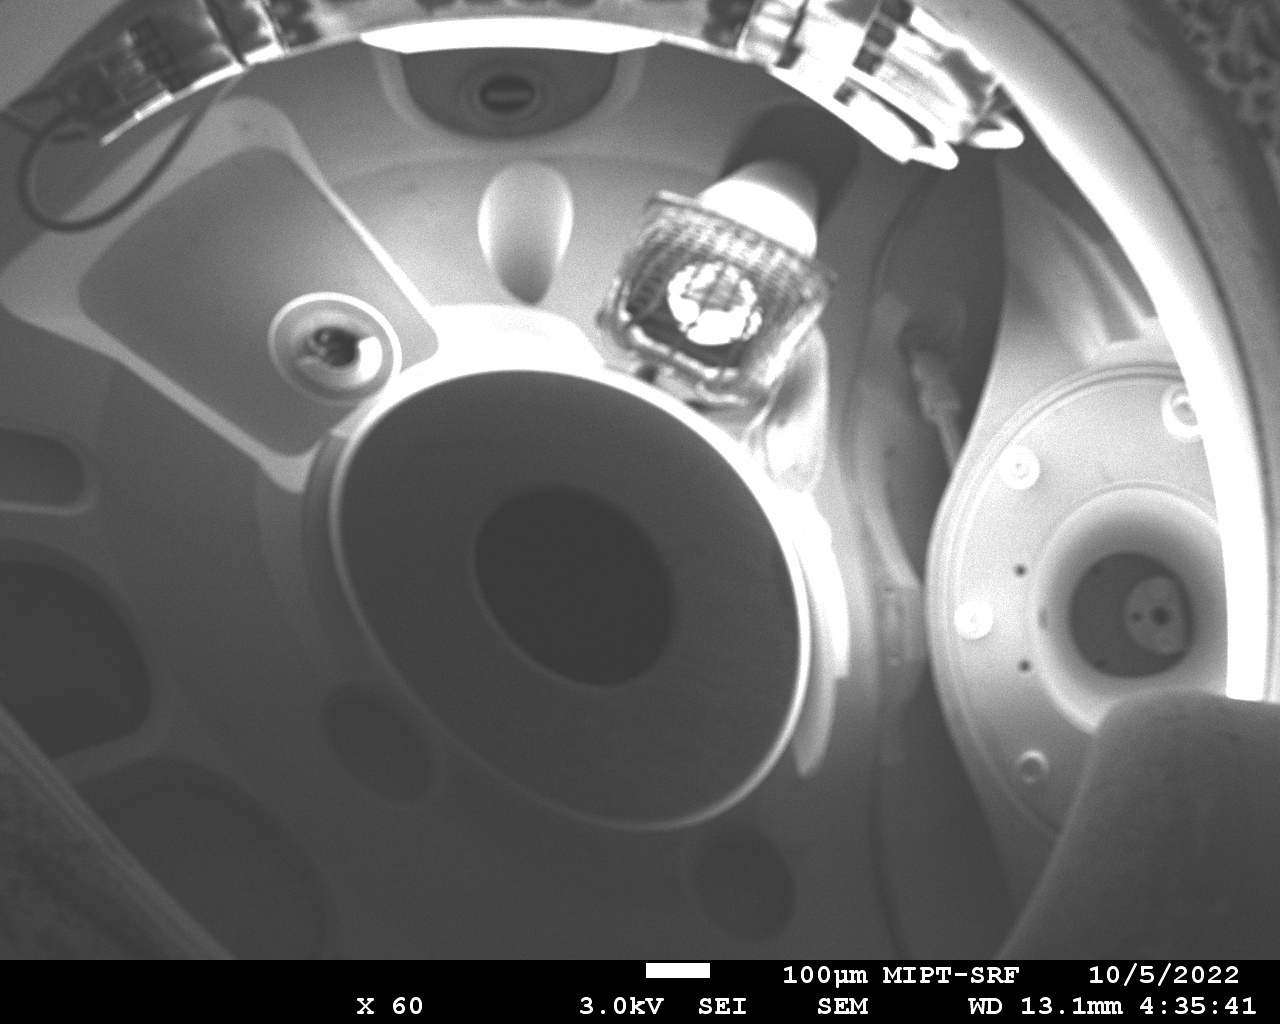
\includegraphics[scale=0.3]{pic15.jpg}
	\caption{Эффект <<Зеркала>>}
	\label{pic15}
\end{figure}

\begin{figure}[H]
	\centering
	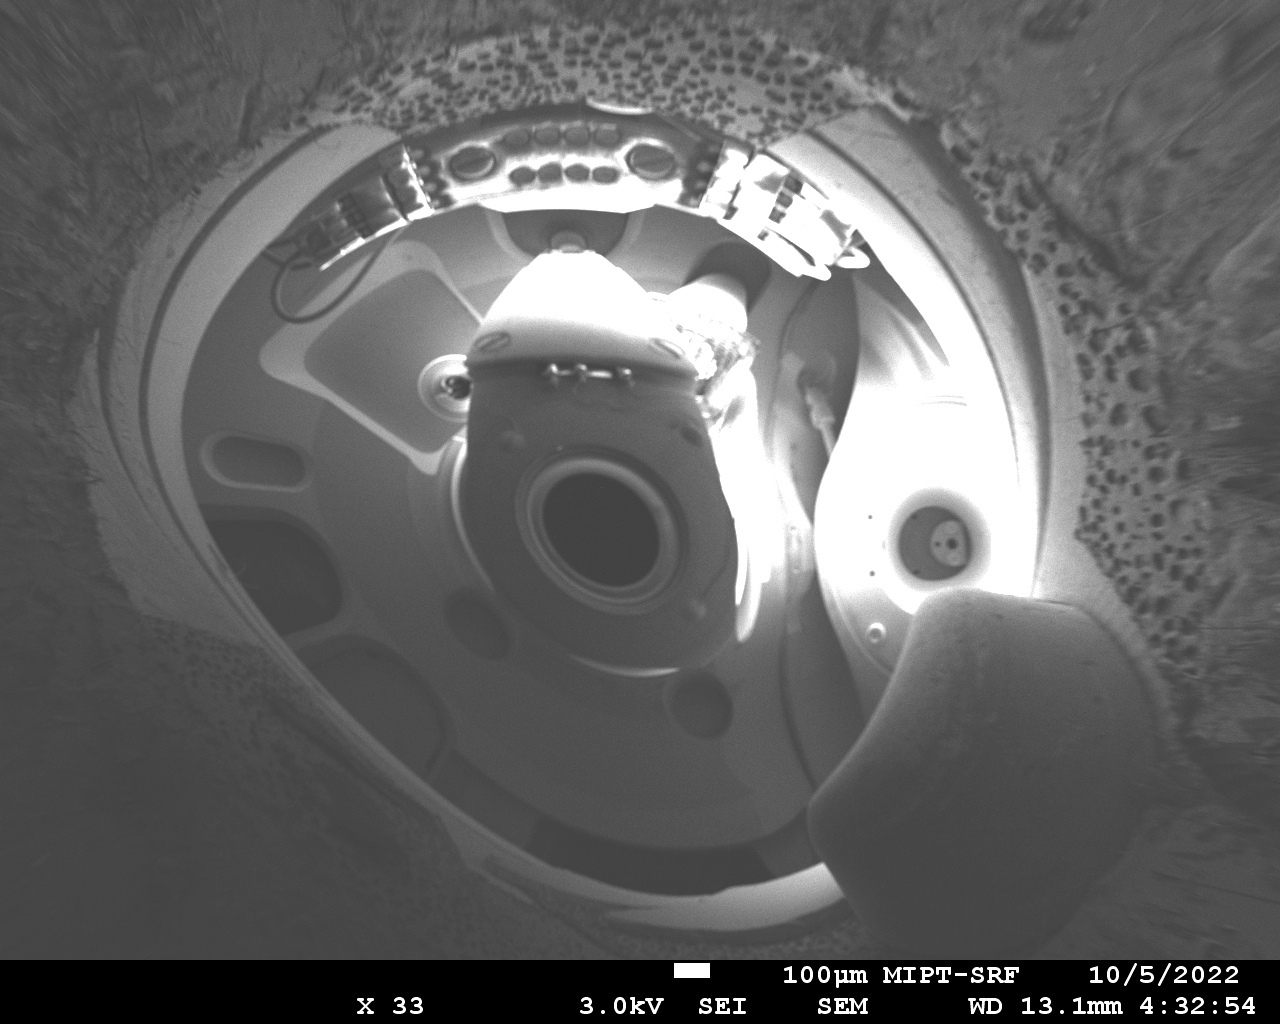
\includegraphics[scale=0.3]{pic16.jpg}
	\caption{Эффект <<Зеркала>>}
	\label{pic16}
\end{figure}


Эффект объясняется тем, что при большой величине накопленного отрицательного заряда электроны первичного пучка не попадают на образец. Т.е. участок образца играет роль зеркала для электронов, что приводит к формированию изображения окружающих деталей камеры микроскопа.






	
	
\end{document}
